\documentclass[11pt,twoside,letterpaper]{book}
\usepackage{longtable}
\usepackage{multirow}
\usepackage{xltxtra}


\usepackage{pdflscape}
\usepackage{etoolbox}
\usepackage{tocloft}

\usepackage[bookmarksnumbered, bookmarksopen=true]{hyperref}
\hypersetup{colorlinks,
  linkcolor=blue,
  linktoc=page}

\usepackage{amsmath}
\usepackage{microtype}
%para codigo fuente
\usepackage{color}
\usepackage{xcolor}
\usepackage{listings}

\usepackage{bookmark}
\bookmarksetup{numbered}

\usepackage{titlesec} %reformatting the chapter headings
\titleformat{\chapter}[block]
{\normalfont\LARGE\bfseries\centering}
{CAPITULO\thechapter: }{0em}{}

\makeatletter
\bookmarksetup{%
  addtohook={%
    \ifnum\toclevel@chapter=\bookmarkget{level}\relax
    \renewcommand*{\numberline}[1]{Capítulo #1: }%
    \fi
  },
}
\makeatother

\renewcommand{\lstlistingname}{Listado}

\lstset{
  basicstyle=\footnotesize\ttfamily,
  language=C++
}

%margenes

%segun guia
\usepackage[top=2cm, bottom=2cm, inner=3cm, outer=2cm]{geometry}

%segun CD de carrera
%\usepackage[top=2.5cm, bottom=2.5cm, inner=3.5cm, outer=2.5cm]{geometry}

% quita la sangria a los parrafos (sin sangria se ve feo :-)
%\setlength{\parindent}{0cm}

% Para tener cabecera y pie de página con un estilo personalizado
\usepackage{fancyhdr}

% Espacio parrafos
\setlength{\parskip}{6pt}

\usepackage{graphicx}
\usepackage{adjustbox}
% Todas las imágenes están en el directorio tp-img:
\newcommand{\imgdir}{includes}
\graphicspath{{\imgdir/}}

\usepackage{fontspec}
\usepackage{polyglossia}
\setmainlanguage{spanish}

\setromanfont[Mapping=tex-text]{Linux Libertine O}
\setsansfont[Mapping=tex-text]{DejaVu Sans}
\setmonofont[Mapping=tex-text]{DejaVu Sans Mono}

\title{Mejoramiento del Proceso de deshidratación mediante la construcción de un sistema de control automático}
\author{Daniel Rodrigo Saguez Tezanos Pinto}
\date{Diciembre, 2015}

\begin{document}
  %
  % caratula
  %
  %para poner bookmark del CD de requisitos
  \bookmark[page=1,level=-2]{INICIO}

  \pagenumbering{Roman} % para comenzar la numeracion de paginas en numeros romanos

  % caratula --------------------------------------------------------------
  \newcommand{\umsslogo}{%
    \adjustbox{valign=t}{
\includegraphics[scale=0.04]{umss}}%
  }
  \newcommand{\fcytlogo}{%
    \adjustbox{valign=t}{
\includegraphics[scale=0.1]{fcyt}}%
  }

  % Carátula:
  \makeatletter
  \begin{titlepage}
    \thispagestyle{empty}

    \begin{tabular}[t]{c p{10cm} c}
      \umsslogo &
      \begin{center}
        \large{\textsc{Universidad Mayor de San Simón }} \\
        \large{\textsc{Facultad de Ciencias y Tecnología }} \\
        \large{\textsc{Carrera de Ingeniería en Informática}}
      \end{center}
      &
      \fcytlogo \\
    \end{tabular}
    \vfill

    \begin{center}
      \huge{\textsc{\@title}}
    \end{center}
    \vspace{0.5cm}

    %\begin{flushright}
    \begin{center}
      \textsc{
        Proyecto de grado, presentado para optar\\
        al Diploma Académico de Licenciatura \\
        en Ingeniería en Informática.
      }
      %\end{flushright}
    \end{center}

    \vfill
    \begin{tabbing}
      \hspace{2cm}\=\+
      \textsc{Presentado por:} \@author    \\
      \\
      \textsc{Tutor:} Msc. Leticia Blanco Coca    \\
      \\
      %\textsc{Cochabamba - Bolivia}\\
      \\
    \end{tabbing}

    \begin{center}
      \textsc{Cochabamba - Bolivia}\\
      \textsc{\@date}
    \end{center}

    \vfill

    %\hrule
    %\vspace{0.2cm}
    %\noindent\small{Trabajo de Grado \hfill}

  \end{titlepage}

  % caratula --------------------------------------------------------------

  %Dedicatoria y agradecimientos
\addcontentsline{toc}{chapter}{Dedicatoria}
\chapter*{}
\begin{flushright}
\textit{Dedicado a \\
    Valery Tamara Saguez Lamas \\
    Cristal Amalia Tezanos Pinto Solares}
    \end{flushright}
\newpage

  \addcontentsline{toc}{chapter}{Agradecimientos}
\chapter*{}
\begin{flushright}
\textit{La realizaci�n de este proyecto de grado \\
        blah blah blah blah blah blah blah blah \\
        blah blah blah blah blah blah blah blah \\
        blah blah blah blah blah blah blah blah \\ 
        blah blah blah blah blah blah blah blah \\
        }
    \end{flushright}
\newpage


  % Las páginas empiezan a contar desde aqui
  \setcounter{page}{1}
  \addcontentsline{toc}{chapter}{Ficha resumen}
\chapter*{Ficha resumen}
Se busca mejorar el proceso de deshidratación de alimentos, mediante la
conjunción de un sistema eléctrico/electrónico, sensores, controladores y
microcontroladores; que permitan tener un seguimiento automático del proceso de
deshidratado, con el fin de monitorear las variables referentes al secado de
diferentes tipos de alimentos; variables como temperatura, velocidad de flujo de
aire, peso, humedad del aire, humedad del producto.
\cleardoublepage

  \bookmark[page=9,level=-1]{�ndice general}
% Pongo el �ndice en una p�gina aparte:
\tableofcontents
\cleardoublepage

  \listoffigures % indice de figuras
\cleardoublepage

  \listoftables % indice de tablas

  \chapter{Introducción}\label{cap:intro}
\pagenumbering{arabic}
\section{Antecedentes}
El  Programa de Alimentos y Productos Naturales (PAPN) fue creado el 13 de
febrero de 1987 como un programa, pero rápidamente se convirtió, por iniciativa
y esfuerzo de su dirección y sus miembros, en un centro superior de
investigación. Este centro depende de la Facultad de Ciencias y Tecnología de la
Universidad Mayor de San Simón (UMSS) y esta situado en el campus principal.
Dentro de sus actividades de ciencia y tecnología en el campo agroalimentario y
de productos naturales, la UMSS ejecuta la investigación a través de convenios y
proyectos en diferentes ámbitos del desarrollo regional y nacional, a través del
centro superior PAPN.

De acuerdo a posibilidades y disponibilidades, se han incorporado al PAPN
practicas sobre secado y análisis sensorial para los estudiantes de ingeniería
industrial y alimentos, así como se han realizado diversos estudios en el secado
de alimentos andinos y el diseño de secadores solares, convencional, deseando
implementar 2 nuevos tipos de deshidratadores: cama fluidizada. y spray.

En este sentido, para mejorar el estudio y la investigación del secado de
alimentos es que este centro precisa la construcción de tres secadores
experimentales automatizados que permitan obtener datos de las variables de
secado de diferentes tipos de alimentos de la forma más rápida y precisa.

El propósito de un control automático en un sistema es producir una salida
deseada cuando las entradas del sistema son modificadas. Estas entradas se
modifican por señales de mando, y también por perturbaciones, que se espera que
el control automático minimice.

%\pagebreak % poner esto al final de cada seccion
\section{Identificación del problema}

Es complicado analizar todas las variables que intervienen en el proceso de
deshidratado, para que, dado un producto que se desea secar; se pueda escoger el
mejor proceso para este producto.

\subsection{Definición del problema}

¿Como mejorar la obtención y almacenamiento de las variables de secado de
distintos tipos de alimentos, por medio del control de las variables de entrada?


\section{Objetivos}

\subsection{Objetivos General}
\begin{itemize}
  \item Construir un sistema de control automático para el proceso de
        deshidratación experimental de alimentos.
  %\item blah blah blah blah.

\end{itemize}

\subsection{Objetivos Específicos}
Los objetivos a cumplir durante el desarrollo del proyecto son:
\begin{itemize}
  \item Determinar el modelo del sistema y de control.
  \item Seleccionar sensores, controladores y actuadores a utilizar.
  \item Desarrollar el modulo para funcionamiento básico del microcontrolador.
  \item Diseñar el modelo unificado el sistema electrónico y el sistema de información.
  \item Desarrollar el modulo de control supervisado.
  \item Desarrollar el modulo de cambio de parámetros de control.
  \item Implementar el control automático.
\end{itemize}

\section{Alcance}
El proyecto tendrá el siguiente alcance:
\begin{itemize}
  \item blah blah blah blah.
  \item blah blah blah blah.
  \item blah blah blah blah.
  \item blah blah blah blah.
  \item blah blah blah blah.
  \item blah blah blah blah.
\end{itemize}


%\pagebreak % poner esto al final de cada seccion
\section{Justificación}
La desecación de vegetales por paso de aire caliente sobre superficie húmeda,
representa la forma mas común de secado de vegetales destinados a la
alimentación, siendo uno de los procesos mas antiguos de conservación que se
conocen.

Mediante este método es posible preservar el color, los principios activos otras
características de calidad que se pierden por acción de las encimas después de
la cosecha, permitiendo de esta manera, una mejor conservación por tiempos
relativamente largos sin perdidas de estas características.

Ante la necesidad de conocer las distintas cualidades y capacidades de los
distintos tipos de deshidratadores, y de obtener los cambios de sus variables
durante el proceso de deshidratación de manera rápida y casi desatendida por una
persona se ve que es conveniente la construcción de un sistema de control
automático para cada tipo de deshidratador que se cuenta en la planta piloto.



  \input{009-Cap02-Deshidratación}
  \input{010-Cap03-ControlAutomático}
  \chapter{Herramientas}
\section{Raspberry Pi}

Raspberry Pi es una computadora de placa de bajo costo que corre GNU/Linux y otros sistemas operativos. Existen dos modelos el A y B, el modelo B tiene la revisión 1 y 2, y además de una nueva versión que es B+.
%TODO aumentar algo mas
\subsection{Componentes}
\begin{itemize}
\item Broadcom BCM2835, SoC que contiene memoria, microprocesador y procesador gráfico.
\item Conector GPIO (Entradas y salidas de propósito general).
\item Conector salida de video compuesto
\item Conector salida de video HDMI
\item LEDs de actividad de LAN y Power
\item Conector de salida de audio
\item Conector microusb para alimentación
\item Circuito integrado para LAN
\item Conectores de expansión (para cámara de video y salida de video)
\item Conectores USB
\item Conector RJ45 para Ethernet
\item Reguladores de voltaje de 1.8v, 2.8v y 3.3v 
\end{itemize}

\begin{figure}
  \centering
    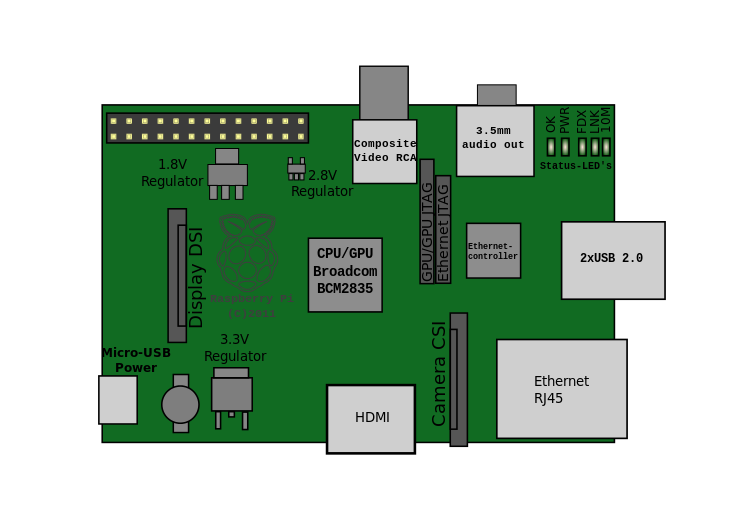
\includegraphics[width=0.5\textwidth]{raspi_pcb}
  \caption{Ubicación de los componentes de Raspberry Pi. \cite{raspberry_pi_wiki}}
  \label{fig:raspi_pcb}
\end{figure}

\begin{table}
\centering
  \begin{tabular}{r r r r}
\textbf{Pin} & \textbf{Descripción} & \textbf{Pin} & \textbf{Descripción} \\
\hline
1 & \texttt{3.3v} & 2 & \texttt{5v} \\
3 & \texttt{SDA0*} & 4 & \texttt{5v} \\
5 & \texttt{SCL0*} & 6 & \texttt{GND} \\
7 &  \texttt{GPIO\_GCLK} & 8 & \texttt{TXD0*} \\
9 &  \texttt{GND} & 10 & \texttt{RXD0*} \\
11 &  \texttt{GPIO\_GEN0} & 12 & \texttt{GPIO\_GEN1} \\
13 &  \texttt{GPIO\_GEN2} & 14 & \texttt{GND} \\
15 &  \texttt{GPIO\_GEN3} & 16 & \texttt{GPIO\_GEN4} \\
17 &  \texttt{3.3v} & 18 & \texttt{GPIO\_GEN5} \\
19 &  \texttt{SPI\_MOSI*} & 20 & \texttt{GND} \\
21 &  \texttt{SPI\_MISO*} & 22 & \texttt{GPIO\_GEN6} \\
23 &  \texttt{SPI\_SCLK*} & 24 & \texttt{SPI\_CEO\_N*} \\
25 &  \texttt{GND} & 26 & \texttt{SPI\_CE1\_N*} \\
  \end{tabular}
  \caption{Descripción de los pines de GPIO}
  \label{table:gpio_descr}
\end{table}

\section{Conclusiones}

blah blah.

  \chapter{Metodolog\'ia}

\section{Pila del producto (product backlog)}
%\section{Pila del producto}
En el presente proyecto se utilizará la metodología de desarrollo de software SCRUM \cite{scrum_book}.

La siguiente tabla es una lista priorizada de requisitos (features) para ser implementadas en el proyecto. Cada una de estas caracteristicas se escribieron de acuerdo a los objetivos específicos, que fueron definidos en el Capitulo \ref{cap:intro}.

\def\arraystretch{2}
\newcommand{\pbesquiv}{Como robot debo ser capaz de esquivar los obstáculos que se presentan en el camino del robot, con el objetivo de hacerlo de forma autónoma. }

\newcommand{\pbplathard}{Como estudiante debo implementar una plataforma de hardware que sirva de base para el robot, con el objetivo de tener un robot operativo.}
\newcommand{\pbrecon}{Como robot quiero ser capaz de reconocer objetos existentes en un fotograma, con el objetivo de tener estos datos para calcular su posición en el plano.}

\newcommand{\pbprof}{Como robot quiero saber a que profundidad en el plano se encuentran los obstáculos, con el objetivo de poder esquivarlos sabiendo su posición.}

\newcommand{\pbdocum}{Como estudiante debo escribir la documentación del proyecto de grado, con el objetivo de tenerlo completado.}

\newcommand{\pbincli}{Como robot quiero saber mi inclinación actual, con el objetivo de saber si estoy en peligro de volcarme.}

\begin{longtable}{|c|p{12.5cm}|c|} %p{1.8cm}|p{1.9cm}
\hline
\textbf{N°} & \textbf{Características (features)} & \textbf{Prioridad} \\ \hline
\hline
%Se diseñará un robot de tal manera que sea totalmente inalámbrico.
%listo

%Se implementará un sistema de visión artificial que sea capaz de reconocer obstáculos existentes en un plano.
1 & \pbrecon & Alta  \\ \hline
%investigar opencv blobs
%investigar filtros
%Obtener coordenadas de objetos reconocidos


%Se implementará un algoritmo para detectar la profundidad de los obstáculos en un fotograma.

2 & \pbprof & Alta \\ \hline
%Obtener distancia aproximada de los objetos reconocidos



%Se implementará un sistema de navegación que permita al robot moverse de forma autónoma a un destino establecido.
%3 & Como robot debo ser capaz de llegar a un destino establecido de forma autónoma, con el objetivo de cumplir las instrucciones del operador. & Alta \\ \hline

3 & \pbesquiv & Alta \\ \hline

4 & \pbplathard & Alta \\ \hline

5 & \pbdocum  & Media \\ \hline


%Se implementará un sistema de comunicaciones entre el robot y el operador.
%7 & Como robot quiero ser capaz de comunicarme con mi operador, con el objetivo de poder recibir coordenadas para saber mi destino. & Media  \\ \hline

% Se desarrollará un sistema de posicionamiento, el cual detectara la posición actual del robot.
%8 & Como robot quiero saber mi posición actual, con el objetivo de poder enviar al robot cuando se sepan las coordenadas. & Media \\ \hline

%Se implementará un sistema de protección que alarme al robot en caso de estar peligrosamente inclinado.
6 & \pbincli  & Baja \\ \hline
% Habilitar giroscopio a raspberry pi
% Implementar sistema de proteccion, deacuerdo con las limitaciones del robot

%Se escribirá documentación técnica y de usuario del software a entregar.
%10 & Como usuario técnico quiero saber como configurar e instalar el sistema, con el objetivo de tener un sistema completamente operativo  & Baja \\ \hline

%11 & Como usuario final quiero saber como operar el robot, con el objetivo de aprender a operar el robot. & Baja \\ \hline
\end{longtable}

\section{Estimaci\'on de historias de usuario}
La estimación de esfuerzo de las historias de usuario se realizaran utilizando la técnica de Planning Poker. Se utilizara el rango de 1, 2, 3, 5, 8, 13.

\section{Sprint A}
El sprint A empieza el d�a Viernes 26 de Septiembre del 2014. Este sprint consta de 2 semanas para completar las historias que ser�n definidas en la planificaci�n del sprint. El sprint concluir� el Jueves 9 de Octubre del 2014.

%\begin{landscape}
\subsection{Sprint backlog}
En este sprint se eligi� trabajar en los features 1 y 2 del product backlog, por el hecho de tener alta prioridad.  Cada feature se divide en historias de usuario, y estas son estimadas con puntos de historia. En los Cuadros \ref{table:eus1} y \ref{table:eus2} se definen las estimaciones. Para cada historia de usuario se definen criterios de aceptaci�n, como se muestra en el Cuadro~\ref{table:criteriosSA}.

Cada historia de usuario se divide en tareas, y se definen en los Cuadros \ref{table:tareasUS1}, \ref{table:tareasUS2} y \ref{table:tareasUS3_1}.

%--------------------------------------------------------------------
\begin{table}[ht]
\centering
\begin{tabular}{|l|p{6cm}|c|p{5cm}|r|}
\hline
\textbf{No.} & \textbf{Feature} & \textbf{Id.} & \textbf{Historia de usuario} & \textbf{Estimaci�n} \\
\hline
1 & \pbrecon & US1 & Obtener coordenadas de objetos reconocidos. & 3 \\ 
\hline
\end{tabular}
\caption{Estimaci�n de US1}
\label{table:eus1}
\end{table}

%--------------------------------------------------------------------
\begin{table}[ht]
\centering
\begin{tabular}{|l|p{6cm}|c|p{5cm}|r|}
\hline
\textbf{No.} & \textbf{Feature} & \textbf{Id.} & \textbf{Historia de usuario} & \textbf{Estimaci�n} \\
\hline
2 & \multirow{2}{6cm}{\pbprof} 
& US2 & Controlar la posici�n de la c�mara. & 3 \\
\cline{3-5}
& & US3 & Obtener distancia aproximada de los objetos reconocidos. & 8 \\
\hline
\end{tabular}
\caption{Estimaci�n de US2 y US3}
\label{table:eus2}
\end{table}


%--------------------------------------------------------------------
\begin{table}[ht]
\centering
\begin{tabular}{|l|p{15cm}|}
\hline
\textbf{Id.} & \textbf{Criterios de aceptaci�n}\\
\hline
US1 & El software a implementar debe ser capaz de reconocer las coordenadas de un objeto en tiempo real, pueden ser de uno o varios objetos captados en el fotograma. \\
\hline
US2 & Dando como entrada el �ngulo con respecto al eje vertical, la c�mara debe ser capaz de posicionarse al �ngulo de entrada establecido. \\
\hline
US3 & Ya teniendo las coordenadas del objeto, el software a implementar debe ser capaz de devolver la distancia que existe entre un objeto y el robot. \\
\hline
\end{tabular}
\caption{Criterios de aceptaci�n del sprint A}
\label{table:criteriosSA}
\end{table}


%--------------------------------------------------------------------
\begin{table}[ht]
\centering
\begin{tabular}{|c|p{13cm}|}
\hline
\textbf{US1} & \textbf{Obtener coordenadas de objetos reconocidos} \\
\hline
\hline
\textbf{Id.} & \textbf{Tareas}\\
\hline
T1 & Preparar estructura simple de archivos para el sistema  \\ \hline
T2 & Investigar acerca OpenCV \\ \hline
T3 & Configurar e instalar OpenCV en Raspberry Pi y en la laptop de trabajo \\ \hline
T4 & Investigar acerca de OpenCVBlobsLib \\ \hline
T5 & Investigar acerca de filtros de OpenCV para el POC \\ \hline
T6 & Implementar POC usando OpenCVBlobsLib \\ \hline
T7 & Escribir funci�n que devuelva coordenadas de los blobs identificados \\ \hline
T8 & Hacer pruebas de la implementaci�n en Raspberry Pi \\ \hline
\end{tabular}
\caption{Tareas del US1}
\label{table:tareasUS1}
\end{table}

%--------------------------------------------------------------------
\begin{table}[ht]
\centering
\begin{tabular}{|c|p{13cm}|}
\hline
\textbf{US2} & \textbf{Controlar la posici�n de la c�mara.} \\
\hline
\hline
\textbf{Id.} & \textbf{Tareas} \\
\hline
T1 & Fabricar soporte motorizado para c�mara \\ \hline
T2 & Implementar funci�n que gira la c�mara a una posici�n especifica \\ \hline
T3 & Escribir y ejecutar prueba de unidad para el m�todo que gira la c�mara \\ \hline
\end{tabular}
\caption{Tareas del US2}
\label{table:tareasUS2}
\end{table}


%--------------------------------------------------------------------
\begin{table}[ht]
\centering
\begin{tabular}{|c|p{13cm}|}
\hline
\textbf{US3} & \textbf{Obtener distancia aproximada de los objetos reconocidos} \\
\hline
\hline
\textbf{Id.} & \textbf{Tareas} \\
\hline
T1 & Deducir f�rmulas para obtener la distancia de los objetos en la pantalla, de acuerdo con el �ngulo de inclinaci�n de la c�mara. \\ \hline
T2 & Implementar funci�n que devuelva distancia de objetos. \\ \hline
\end{tabular}
\caption{Tareas del US3}
\label{table:tareasUS3_1}
\end{table}
%--------------------------------------------------------------------

\subsection{Reconocimiento de objetos utilizando OpenCV}\label{sec:recopencv}
El sistema de reconocimiento de objetos ejecuta una serie de pasos antes de enviar un fotograma al reconocimiento de blobs. Primero se ejecuta \texttt{dilate()}, para remover peque�os puntos en la imagen, que no son relevantes para este caso. Segundo se ejecuta \texttt{Canny()}, que devuelve una imagen con bordes delgados y finos. Una vez ejecutados estos pasos se env�a la imagen resultado a \texttt{CBlobresult()}, que devuelve los blobs detectados en la imagen. Todo este proceso se puede apreciar en la Figura~\ref{fig:opencvproc}.

El resultado de \texttt{CBlobresult()} es un conjunto de blobs. Cada elemento del conjunto contiene datos como ser: el �rea, coordenadas de la posici�n, dimensiones, etc. 
%Algunos datos de este conjunto de blobs resultado es enviado al sistema experto como datos de entrada.

\begin{figure}
  \centering
    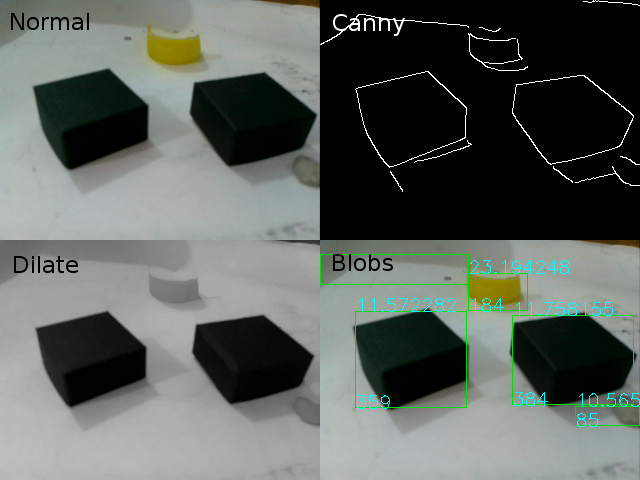
\includegraphics[width=0.5\textwidth]{opencvproc}
  \caption{Reconocimiento de objetos utilizando OpenCV. Elaboraci�n propia.}
  \label{fig:opencvproc}
\end{figure}

\subsection{Control del servomotor de la c�mara}
La c�mara estar� montada a un servomotor y este al robot, de manera que ser� posible mover la c�mara en el eje vertical como se muestra en la Figura~\ref{fig:servo}.

\begin{figure}
  \centering 
    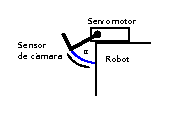
\includegraphics[width=0.5\textwidth]{servo}
  \caption{C�mara y servomotor montados al Robot. Elaboraci�n propia.}
  \label{fig:servo}
\end{figure}
%https://github.com/richardghirst/PiBits/tree/master/ServoBlaster
Ya teniendo al servomotor y a la c�mara montados, es necesario poder controlarlos. El servomotor recibe n�meros para poder moverlo, la forma de poder enviar n�meros es mediante un archivo especial llamado \texttt{/dev/servoblaster}. ServoBlaster es una interfaz para controlar servomotores mediante los pines de GPIO. Los n�meros que recibe ServoBlaster son ancho de pulsos, luego estos datos son transmitidos mediante el GPIO hasta el servomotor. Para poder mover la c�mara a un cierto �ngulo con respecto al eje vertical, es necesario transformar los anchos de pulsos a grados, para esta transformaci�n se utilizar� la t�cnica de interpolaci�n de Lagrange \cite{ipolinomica}.

\begin{equation}
p(x) = \sum_{i=0}^{n}\left(\prod_{\substack{0 \leq j \leq n \\ j \neq i}}{\frac{x - x_j}{x_i - x_j}}\right) * y_i \label{lagrange}
\end{equation}

Se utilizaran tres puntos, que cada uno es el �ngulo en grados (con respecto al eje vertical como se muestra en la Figura~\ref{fig:servo}) con su correspondiente ancho de pulso. Estos puntos se muestran en el Cuadro~\ref{table:puntosg2pwm}.

\begin{table}
\centering
\begin{tabular}{| r | r | r |}
\hline
  & \textbf{x} & \textbf{y} \\
\hline
0 & 180 & 89 \\ 
\hline
1 &  90 & 189 \\
\hline
2 &  45 & 242 \\
\hline
\end{tabular}
\caption{Conversi�n de grados a modulaci�n por ancho de pulso}
\label{table:puntosg2pwm}
\end{table}

Luego reemplazando en \ref{lagrange} se obtiene la Ecuaci�n~\ref{servolagr}.

%p(x) =  \frac{(x - 90) * (x - 45)}{12150} * 89 + \\
%        \frac{(x - 180) * (x - 45)}{-4050} * 189 + \\
%        \frac{(x - 180) * (x - 90)}{-6075} * 242 \label{servolagr}

\begin{equation}
p(x) = \frac{(x - x_1) * (x - x_2) * y_0}{(x_0 - x_1) * (x_0 - x_2)} + \frac{(x - x_0) * (x - x_2) * y_1}{(x_1 - x_0) * (x_1 - x_2)} + \frac{(x - x_0) * (x - x_1) * y_2}{(x_2 - x_0) * (x_2 - x_1)} \label{servolagr} 
\end{equation}

En la Ecuaci�n~\ref{servolagr}, $x$ representa el �ngulo de entrada, y el resultado de $p(x)$ es el ancho de pulso. Con este dato ya es posible indicar al servomotor cuanto se debe mover para posicionar la c�mara al �ngulo $x$, que seria $\alpha$ en la Figura~\ref{fig:servo}.

\subsection{Casos de prueba}


\begin{longtable}{|l|p{10cm}|}
\hline
\textbf{Id.} & CP1 \\
\hline
\textbf{Historia} & US1\\
\hline
\textbf{Nombre} & Prueba de funcionamiento de ambiente de desarrollo \\
\hline
\textbf{Descripci�n} & Se realizar�n pruebas de OpenCV de los ambientes de desarrollo de Raspberry Pi, para verificar que OpenCV y las herramientas de desarrollo est�n correctamente instaladas \\
\hline
\textbf{Ambiente de prueba} & Raspberry Pi con Raspbian y OpenCV \\
\hline
\textbf{Inicializaci�n} & Encender Raspberry Pi\\
\hline
%\textbf{Finalizaci�n} & Ninguna\\
%\hline
\textbf{Acciones} &  
\parbox[][][s]{8cm}{ 
            \begin{itemize}
                \item Copiar \texttt{opencv-2.4.9.zip} al Raspberry Pi
                \item Descomprimir \texttt{opencv-2.4.9.zip}
                \item Entrar a opencv-2.4.9/samples/cpp
                \item Ejecutar \texttt{\$ g++ `pkg-config --libs --cflags opencv` houghlines.cpp -o houghlines}
                \item Ejecutar \texttt{./houghlines}
            \end{itemize} 
}
\\
\hline
\textbf{Salida esperada} & Dos ventanas gr�ficas con t�tulos ``source'' y ``detected lines''. La segunda ventana tiene los bordes marcados con rojo.\\
\hline
\textbf{Salida obtenida} & En la Figura~\ref{fig:houghlinesRes} se muestra la salida obtenida de Houghlines, que es una transformada usada para detectar lineas rectas. \\
\hline
\textbf{Resultado} & \textbf{Correcto}\\
\hline
\end{longtable}

\begin{figure}
  \centering
    
\includegraphics[width=0.5\textwidth]{houghlines}
  \caption{Salida de ejecuci�n de Houghlines. Elaboraci�n propia.}
  \label{fig:houghlinesRes}
\end{figure}

%----------------------

\begin{longtable}{|l|p{10cm}|}
\hline
\textbf{Id.} & CP2 \\
\hline
\textbf{Historia} & US1\\
\hline
\textbf{Nombre} & Prueba de funcionamiento de ambiente de desarrollo en laptop de trabajo \\
\hline
\textbf{Descripci�n} & Se realizar�n pruebas de OpenCV de los ambientes de desarrollo de la laptop de trabajo, para verificar que OpenCV y las herramientas de desarrollo est�n correctamente instaladas. \\
\hline
\textbf{Ambiente de prueba} & Laptop de trabajo y OpenCV \\
\hline
\textbf{Inicializaci�n} & Ninguna\\
\hline
%\textbf{Finalizaci�n} & Ninguna\\
%\hline
\textbf{Acciones} &  
\parbox[][][s]{8cm}{ 
            \begin{itemize}
                \item Encender laptop y entrar a la terminal.
                \item Copiar \texttt{opencv-2.4.9.zip} a directorio.
                \item Descomprimir \texttt{opencv-2.4.9.zip}
                \item Entrar a opencv-2.4.9/samples/cpp
                \item Ejecutar \texttt{\$ g++ `pkg-config --libs --cflags opencv` houghlines.cpp -o houghlines}
                \item Ejecutar \texttt{./houghlines}
            \end{itemize} 
}
\\
\hline
\textbf{Salida esperada} & Dos ventanas gr�ficas con t�tulos ``source'' y ``detected lines''. La segunda ventana tiene los bordes marcados con rojo.\\
\hline
\textbf{Salida obtenida} & En la Figura~\ref{fig:houghlinesLap} se muestra la salida obtenida de Houghlines, que es una transformada usada para detectar lineas rectas.\\
\hline
\textbf{Resultado} & \textbf{Correcto}\\
\hline
\end{longtable}

\begin{figure}
  \centering
    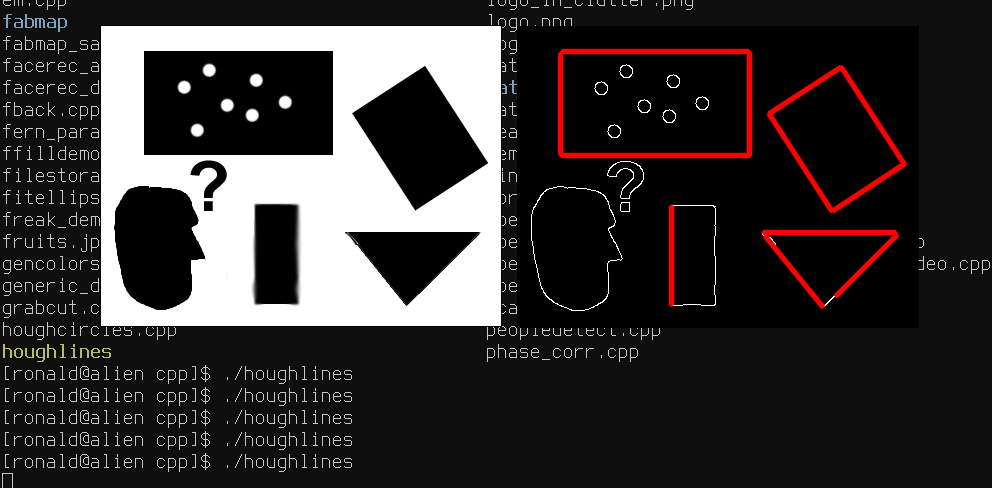
\includegraphics[width=0.5\textwidth]{houghlinesLap}
  \caption{Salida de ejecuci�n de Houghlines. Elaboraci�n propia.}
  \label{fig:houghlinesLap}
\end{figure}

%---------------------------

\begin{longtable}{|l|p{10cm}|}
\hline
\textbf{Id.} & CP3 \\
\hline
\textbf{Historia} & US1\\
\hline
\textbf{Nombre} & Prueba de funcionamiento de \texttt{Blobs::findBlobs} \\
\hline
\textbf{Descripci�n} & Se realizar�n pruebas de \texttt{Blobs::findBlobs}, para verificar que este m�todo encuentra regiones (blobs) en una imagen dada. \\
\hline
\textbf{Ambiente de prueba} & Computadora con OpenCV, herramientas de desarrollo y c�digo fuente del proyecto. \\
\hline
\textbf{Inicializaci�n} & Ninguna \\
\hline
%\textbf{Finalizaci�n} & Ninguna \\
%\hline
\textbf{Acciones} &  
\parbox[][][s]{8cm}{ 
            \begin{itemize}
                \item Ingresar a la computadora de desarrollo
                \item Ir al directorio sistema/unit\_tests
                \item Ejecutar la compilaci�n de la prueba de unidad: \texttt{\$ make test\_find\_blobs}
                \item El anterior paso deber�a generar test\_find\_blobs
                \item Ejecutar \texttt{./test\_find\_blobs}
            \end{itemize} 
}
\\
\hline
\textbf{Salida esperada} & Una ventana gr�fica con una foto de tres objetos negros, cada objeto con un recuadro verde.\\
\hline
\textbf{Salida obtenida} & En la Figura~\ref{fig:testBlobsRes} se muestra la salida obtenida. El m�todo \texttt{GetNumBlobs()} usado aqu�, se ocupa de detectar objetos en una imagen dada.\\
\hline
\textbf{Resultado} & \textbf{Correcto}\\
\hline
\end{longtable}

\begin{figure}
  \centering
    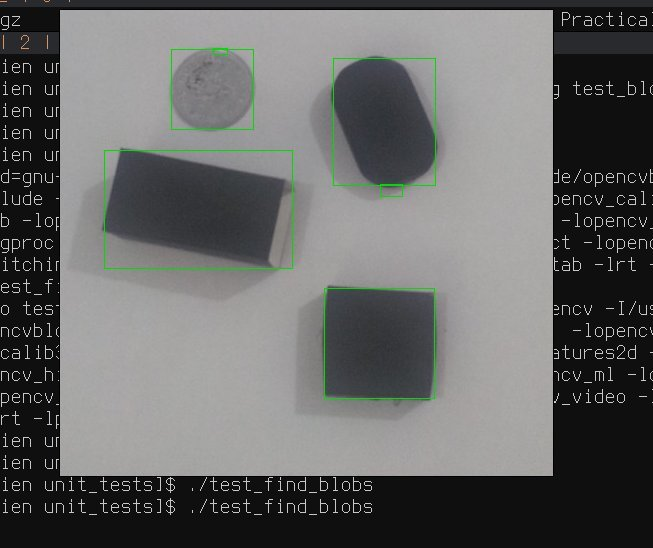
\includegraphics[width=0.5\textwidth]{testBlobsRes}
  \caption{Salida de ejecuci�n de \texttt{./test\_find\_blobs}.  Elaboraci�n propia.}
  \label{fig:testBlobsRes}
\end{figure}

%---------------------------

\begin{longtable}{|l|p{10cm}|}
\hline
\textbf{Id.} & CP4 \\
\hline
\textbf{Historia} & US1\\
\hline
\textbf{Nombre} & Prueba de funcionamiento de coordenadas de \texttt{Blobs::findBlobs} \\
\hline
\textbf{Descripci�n} & Se realizar�n pruebas para verificar que las coordenadas que devuelve \texttt{Blobs::findBlobs} sean correctas \\
\hline
\textbf{Ambiente de prueba} & Computadora con OpenCV, herramientas de desarrollo, c�digo fuente del proyecto, y GIMP \\
\hline
\textbf{Inicializaci�n} & Ninguna \\
\hline
%\textbf{Finalizaci�n} & Ninguna \\
%\hline
\textbf{Acciones} &  
\parbox[][][s]{8cm}{ 
            \begin{itemize}
                \item Ingresar a la computadora de desarrollo
                \item Ir al directorio sistema/unit\_tests
                \item Ejecutar la compilaci�n de la prueba de unidad: \texttt{\$ make test\_find\_blobs}
                \item El anterior paso deber�a generar test\_find\_blobs
                \item Ejecutar \texttt{./test\_find\_blobs}
                \item Verificar que todas las coordenadas listadas en la salida del programa sean las mismas que los recuadros verdes. Esto se puede realizar con la ayuda de GIMP.
            \end{itemize} 
}
\\
\hline
\textbf{Salida esperada} & Salida en la interfaz de linea de comandos con las coordenadas marcadas en la ventana gr�fica. En esta ventana debe mostrar una foto de tres objetos negros, cada objeto con un recuadro verde. (Es posible que se muestren otros recuadros verdes en otras regiones, esto es completamente normal.)\\
\hline
\textbf{Salida obtenida} & En la Figura~\ref{fig:test_blob_coord} se muestra la salida obtenida. El m�todo \texttt{GetNumBlobs()} tambi�n devuelve las coordenadas de los objetos detectados (blobs).\\
\hline
\textbf{Resultado} & \textbf{Correcto}\\
\hline
\end{longtable}

\begin{figure}
  \centering
    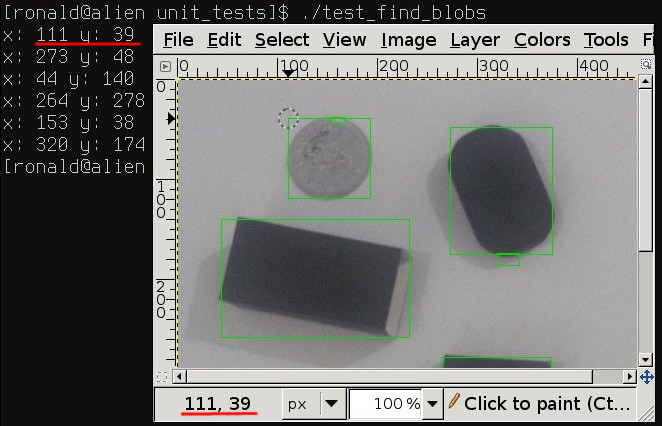
\includegraphics[width=0.5\textwidth]{test_blob_coord}
  \caption{Salida de \texttt{./test\_find\_blobs} mostrando las coordenadas de los blobs. Elaboraci�n propia.}
  \label{fig:test_blob_coord}
\end{figure}


%---------------------------

\begin{longtable}{|l|p{10cm}|}
\hline
\textbf{Id.} & CP5 \\
\hline
\textbf{Historia} & US2\\
\hline
\textbf{Nombre} & Prueba de posicionamiento de la c�mara\\
\hline
\textbf{Descripci�n} & Se realizar�n pruebas para verificar que la c�mara este correctamente posicionada seg�n el software implementado. \\
\hline
\textbf{Ambiente de prueba} & Raspberry Pi con OpenCV, c�mara de Raspberry Pi, herramientas de desarrollo, c�digo fuente del proyecto, y un transportador. \\
\hline
\textbf{Inicializaci�n} & Conectar la c�mara a Raspberry Pi. Marcar una hoja desde 40 grados hasta 180 grados.\\
\hline
%\textbf{Finalizaci�n} & Ninguna\\
%\hline
\textbf{Acciones} &  
\parbox[][][s]{8cm}{ 
            \begin{itemize}
                \item Ingresar al Raspberry Pi
                \item Ir al directorio sistema/unit\_tests
                \item Ejecutar la compilaci�n de la prueba de unidad: \texttt{\$ make test\_servo}
                \item Verificar que el anterior paso genero test\_servo
                \item Ejecutar \texttt{./test\_servo}
                \item Con la hoja marcada, verificar que la c�mara este correctamente alineada seg�n los grados que se muestran en la pantalla.
            \end{itemize} 
}
\\
\hline
\textbf{Salida esperada} & Los grados de la hoja deben coincidir con los grados mostrados en la salida del programa.\\
\hline
\textbf{Salida obtenida} & En la Figura~\ref{fig:test_camara_calib} se muestra la salida obtenida. En la figura se puede obsevar a la c�mara alineada a 90 grados.\\
\hline
\textbf{Resultado} & \textbf{Correcto}\\
\hline
\end{longtable}

\begin{figure}
  \centering
    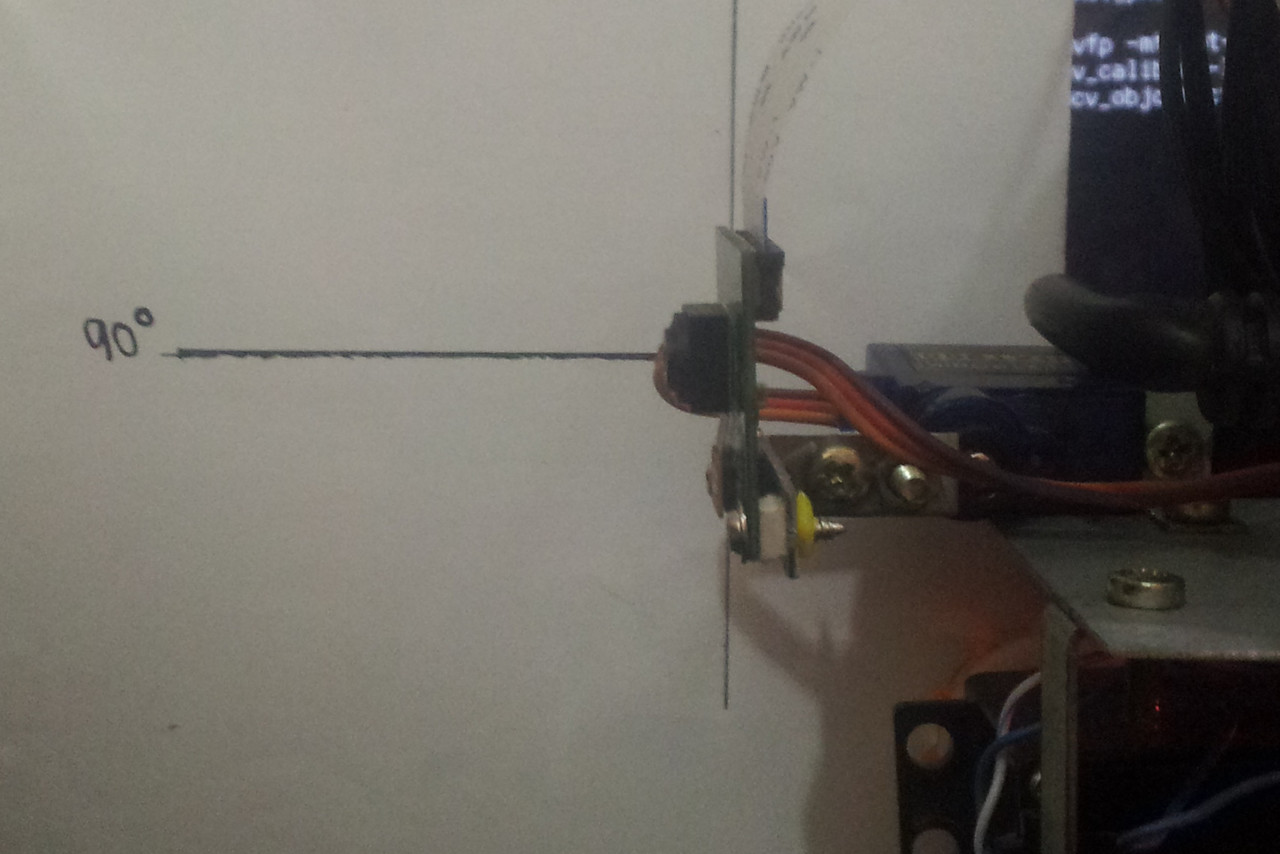
\includegraphics[width=0.5\textwidth]{test_camara_calib}
  \caption{C�mara alineada a 90 grados. Elaboraci�n propia.}
  \label{fig:test_camara_calib}
\end{figure}

\subsection{Demostraci�n de fin de sprint}
 
El m�todo \texttt{findBlobs()} encuentra blobs en una imagen dada (\texttt{im}). En la Figura~\ref{fig:test_blob_coord} se observa las coordenadas de los objetos reconocidos.

\begin{lstlisting}[label=findBlobs,caption=M�todo para encontrar blobs en una imagen]
CBlobResult Blobs::findBlobs(Mat im){
    Mat img, imgc, imgd;

    cvtColor(im,img,CV_BGR2GRAY);
    Mat st_elem = getStructuringElement(MORPH_RECT, Size(size_slider, size_slider));
    dilate(img, imgd, st_elem);

    Canny(imgd, imgc, canny_th1, canny_th2);

    return CBlobResult(imgc,Mat(),NUMCORES);
}
\end{lstlisting}


El m�todo \texttt{addBlobToImg()} a�ade un rect�ngulo al objeto reconocido (blob). Este m�todo recibe como par�metros de entrada, una imagen \texttt{im} y un blob \texttt{t2}. Se obtienen las coordenadas de \texttt{t2} y se utiliza la funci�n \texttt{rectangle} para a�adir el rect�ngulo a la imagen \texttt{im}. En la Figura~\ref{fig:testBlobsRes} se observa que cuatro objetos son reconocidos y encuadrados.


\begin{lstlisting}[label=addBlobToImg,caption=M�todo para a�adir rectangulos a blobs]
Mat Blobs::addBlobToImg(Mat im, CBlob t2){

    Scalar mean, stddev;
        
    Rect bbox = t2.GetBoundingBox();
    rectangle(im,bbox,Scalar(0,220,0),1);
    
    return im;
}

\end{lstlisting}


El m�todo \texttt{mover()} mueve el servomotor a un \texttt{�ngulo} de entrada especificado.
\begin{lstlisting}[label=mover,caption=M�todo para mover un servomotor]
void Servo::mover(double angulo){
    FILE * pFile;

    int servo_a = (int) interpolacion(angulo);
    
    string s = std::to_string(servo_a);
    s = SERVO_NUM + s + "\n";
    const char *cstr = s.c_str();
    
    cout << "Servo: " << s << endl;

    if(enable){
        pFile = fopen (SERVO_FILE, "wb");
        if (pFile != NULL){
            fwrite (cstr , sizeof(char), s.size(), pFile) ;
            fclose (pFile);
        }else{
            cout << "No se puede abrir " << SERVO_FILE << endl;
        }
    }
}
\end{lstlisting}

Utilizando la Ecuaci�n~\ref{servolagr} se implementa el m�todo de \texttt{interpolacion()}.

\begin{lstlisting}[label=interpolacion,caption=M�todo para transformar de grados a modulaci�n por ancho de pulso.]
double Servo::interpolacion(double x){
    
    double x0 = 180, y0 = 89;
    double x1 = 90, y1 = 189;
    double x2 = 45, y2 = 242;

    double y;

    y = ((x - x1) * (x - x2) * y0)/((x0 - x1) * (x0 - x2)) + 
        ((x - x0) * (x - x2) * y1)/((x1 - x0) * (x1 - x2)) + 
        ((x - x0) * (x - x1) * y2)/((x2 - x0) * (x2 - x1));

    return y;
}

\end{lstlisting}

\subsection{Gr�fico burn down del sprint}
La Figura~\ref{fig:sprintA} muestra el gr�fico \emph{burn down} del presente sprint.

\begin{figure}
  \centering
    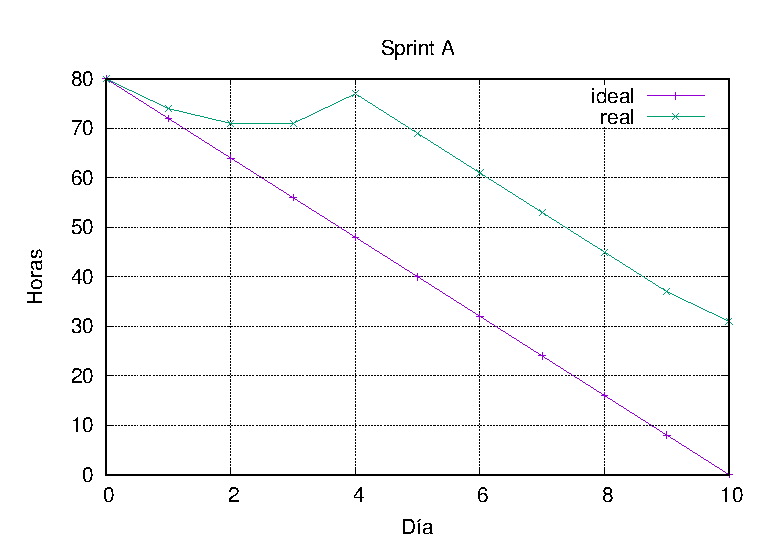
\includegraphics[width=0.5\textwidth]{sprintA}
  \caption{Gr�fico burn down del sprint. Elaboraci�n propia.}
  \label{fig:sprintA}
\end{figure}

\subsection{Retrospectiva del sprint}
\begin{itemize}
  \item �Qu� sali� bien?
    \begin{itemize}
        \item Se completaron la mayoria de las tareas de la iteraci�n.
        \item Se escribieron pruebas de unidad para el c�digo desarrollado.
    \end{itemize}

  \item �Qu� podr�a haber sido mejor?
    \begin{itemize}
        \item La estimaci�n de la historia US3 no fue buena.
    \end{itemize}

  \item �Qu�  se puede mejorar en el futuro?
    \begin{itemize}
        \item Mejorar las estimaciones de las historias, si la historia es muy larga es mejor dividirla.
    \end{itemize}
\end{itemize}





  \chapter{Conclusiones y Recomendaciones}
\section{Conclusiones}

blah blah blah blah blah blah blah blah blah blah blah blah blah blah blah blah blah blah blah blah  blah blah blah blah blah blah blah blah blah blah blah blah blah blah blah blah blah blah blah blah blah blah blah blah blah blah blah blah blah blah blah blah blah blah blah blah blah blah blah blah blah blah blah blah blah blah blah blah blah blah blah blah blah blah blah blah blah blah blah blah blah blah blah blah blah blah blah blah blah blah blah blah blah blah blah blah blah blah blah blah blah blah blah blah blah blah blah blah blah blah blah blah blah blah blah blah blah blah blah blah blah blah blah blah blah blah blah blah blah blah blah blah blah blah blah blah blah blah blah blah blah blah blah blah blah blah blah blah blah blah blah blah blah blah blah blah blah blah blah blah blah blah blah blah blah blah blah blah blah blah blah blah blah blah blah blah blah blah blah blah blah blah blah blah blah blah blah blah blah blah blah blah blah blah blah blah blah blah blah blah 

\section{Recomendaciones}


blah blah blah blah blah blah blah blah blah blah blah blah blah blah blah blah blah blah blah blah  blah blah blah blah blah blah blah blah blah blah blah blah blah blah blah blah blah blah blah blah blah blah blah blah blah blah blah blah blah blah blah blah blah blah blah blah blah blah blah blah blah blah blah blah blah blah blah blah blah blah blah blah blah blah blah blah blah blah blah blah blah blah blah blah blah blah blah blah blah blah blah blah blah blah blah blah blah blah blah blah blah blah blah blah blah blah blah blah blah blah blah blah blah blah blah blah blah blah blah blah blah blah blah blah blah blah blah blah blah blah blah blah blah blah blah blah blah blah blah blah blah blah blah blah blah blah blah blah blah blah blah blah blah blah blah blah blah blah blah blah blah blah blah blah blah blah blah blah blah blah blah blah blah blah blah blah blah blah blah blah blah blah blah blah blah blah blah blah blah blah blah blah blah blah blah blah blah blah blah blah 


\section{Posibles extensiones}


blah blah blah blah blah blah blah blah blah blah blah blah blah blah blah blah blah blah blah blah  blah blah blah blah blah blah blah blah blah blah blah blah blah blah blah blah blah blah blah blah blah blah blah blah blah blah blah blah blah blah blah blah blah blah blah blah blah blah blah blah blah blah blah blah blah blah blah blah blah blah blah blah blah blah blah blah blah blah blah blah blah blah blah blah blah blah blah blah blah blah blah blah blah blah blah blah blah blah blah blah blah blah blah blah blah blah blah blah blah blah blah blah blah blah blah blah blah blah blah blah blah blah blah blah blah blah blah blah blah blah blah blah blah blah blah blah blah blah blah blah blah blah blah blah blah blah blah blah blah blah blah blah blah blah blah blah blah blah blah blah blah blah blah blah blah blah blah blah blah blah blah blah blah blah blah blah blah blah blah blah blah blah blah blah blah blah blah blah blah blah blah blah blah blah blah blah blah blah blah blah 



  \begin{thebibliography}{99}
%\bibitem{Libro_ejemplo} Apellido, Nombre.Nombre texto.Editorial.A�o.# de pag
\bibitem{opencv_cookbook} Lagani�re, Robert.OpenCV 2 Computer Vision Application Programming Cookbook.Packt Publishing.2011.P\'agina 1
\bibitem{raspi_evilg} Norris, Donald.Raspberry Pi Projects for the Evil Genius.Mc Graw Hill.2014 . P�gina 22
\bibitem{prac_rob} Sahin, Ferat; Kachroo, Pushkin . Practical and Experimental Robotics . CRC Press . 2008 . P�gina 43
\bibitem{l298_data} STMicroelectronics . L298 DUAL FULL-BRIDGE DRIVER Datasheet. STMicroelectronics . 2000 . P�gina 2
\bibitem{comp_cv} J�hne, Bernd; Hau�ecker, Horst .  Computer Vision and Applications . Academic Press . 2000 . P�gina 1
\bibitem{appl_cmv} E. R. Davies . Computer and Machine Vision: Theory, Algorithms, Practicalities . Academic Press . 2012 . P�gina 10
\bibitem{modulosocv} Brahmbhatt, Samarth . Practical OpenCV . APress . 2013 . P�gina 22
\bibitem{tomografia} Nixon, Mark; Aguado, Alberto . Feature Extraction and Image Processing . Newnes . 2002 . P�gina 2
\bibitem{resonancia} Davies, E. Roy . Machine Vision: Theory, Algorithms, Practicalities . Morgan Kaufmann . 2005 . P�gina 53
\bibitem{interpolacion} Cyganek, Boguslaw; Siebert, J. Paul; An introduction to 3D computer vision techniques and algorithms . Wiley . 2009 . P�gina 412
\bibitem{noisereduc} E. R. Davies . Computer and Machine Vision: Theory, Algorithms, Practicalities . Academic Press . 2012 . P�gina 40
\bibitem{features} Nixon, Mark; Aguado, Alberto . Feature Extraction and Image Processing . Newnes . 2002 . P�gina 99
\bibitem{egomotion} Burger, Wilhelm; Bhanu, Bir . Estimating 3-D Egomotion from Perspective Image Sequences . IEEE . 2002 . P�gina 1
\bibitem{tracking} Lyudmila MIHAYLOVA; Paul BRASNETT; Nishan CANAGARAJAH; David BULL . Object Tracking by Particle Filtering Techniques in Video Sequences . Department of Electrical and Electronic Engineering, University of Bristol, UK . . P�gina 1
\bibitem{edgedetection} E. R. Davies . Computer and Machine Vision: Theory, Algorithms, Practicalities . Academic Press . 2012 . P�gina 112
\bibitem{cidetection} E. R. Davies . Computer and Machine Vision: Theory, Algorithms, Practicalities . Academic Press . 2012 . P�gina 149
\bibitem{camara} Wenczel, Norma .  Inside the Camera Obscura � Optics and Art under the Spell of the Projected Image . Max Planck Institute for the History of Science . 2007 . P�gina 13-30
\bibitem{luz_visible} Starr, Cecie . Biology: Concepts and Applications . Thomson Brooks/Cole . 2005 . P�gina 94
\bibitem{appl_cv} J�hne, Bernd y Hau�ecker, Horst . Computer Vision and Applications, A Guide for Students and Practitioners . Academic Press . 2000 . P�gina 564
\bibitem{cv_tasks} J�hne, Bernd y Hau�ecker, Horst . Computer Vision and Applications, A Guide for Students and Practitioners . Academic Press . 2000 . P�gina 7
\bibitem{filtros} Bhat, Pravin . Gradientshop: A gradient-domain optimization framework for image and video filtering . ACM Transactions on Graphics . 2010 . P�gina 10  
\bibitem{restauracion} M. Bertalm�o, G. Sapiro, V. Caselles and C. Ballester. Image Inpainting . Proceedings of SIGGRAPH 2000 . 2000 . P�gina 1 
\bibitem{ipolinomica}  Agarwal, R.P.; Wong, J.Y. Patricia . Error Inequalities in Polynomial Interpolation and Their Applications . Springer Science+Bussiness Media, B.V. 1993 . P�gina 217
\bibitem{burndown} Cohn, Mike . User Stories Applied, for Agile Software Development . Addison-Wesley . 2004 . P�gina 121

%\bibitem{} . . . . P�gina 

%\bibitem{PHP} PHP Web-Seite: \url{http://www.php.net}

%\bibitem{robotica_wiki} Rob�tica - Wikipedia: \url{http://es.wikipedia.org/wiki/Rob�tica}. 25 de Marzo de 2014
\bibitem{robotica_wiki} Bermejo, Sergi . Desarrollo de robots basados en el comportamiento . Ediciones UPC . 2003 . P�ginas 26, 27
%\bibitem{opencv_wiki} OpenCV - Wikipedia: \url{http://en.wikipedia.org/wiki/OpenCV}. 25 de Marzo de 2014
\bibitem{scrum_book} Sutherland, Jeff . The Scrum Handbook . Scrum, Inc . 2001 . P�gina 6
\bibitem{opencv_oficial} P�gina oficial de OpenCV: \url{http://opencv.org/}. 27 de Marzo de 2014
\bibitem{raspberry_pi} P�gina oficial de Raspberry Pi: \url{http://www.raspberrypi.org/}. 27 de Marzo de 2014
\bibitem{raspberry_pi_wiki} Componentes de Raspberry Pi: \url{https://www.raspberrypi.org/blog/new-graphic/}. 8 de Septiembre de 2015
%\bibitem{single_board_pc} Single board computer - Wikipedia: \url{https://en.wikipedia.org/wiki/Single-board_computer}. 27 de Marzo de 2014
%\bibitem{reg_voltaje} Regulador de tensi�n: \url{https://es.wikipedia.org/wiki/Regulador_de_tensi\%C3\%B3n}. 11 de Septiembre de 2014
%\bibitem{bateria} Bater�a de ion de litio \url{https://es.wikipedia.org/wiki/Bater\%C3\%ADa_de_ion_de_litio}. 11 de Septiembre de 2014 
\bibitem{camera_mod} Raspberry Pi camera module: \url{http://www.raspberrypi.org/products/camera-module/}. 11 de Septiembre de 2014
\bibitem{cam_espec} Raspberry Pi camera module stock lens characteristics \url{http://www.truetex.com/raspberrypi} . 9 de Octubre de 2014
%\bibitem{camara} C�mara oscura \url{http://es.wikipedia.org/wiki/C\%C3\%A1mara_oscura} . 19 de octubre de 2014
%\bibitem{luz_visible} Radiaci�n electromagn�tica - Wikipedia\url{http://es.wikipedia.org/wiki/Radiaci\%C3\%B3n\_electromagn\%C3\%A9tica#Luz_visible} . 19 de octubre de 2014
%\bibitem{appl_cv} Applications for computer vision - Wikipedia \url{http://en.wikipedia.org/wiki/Computer_vision#Applications_for_computer_vision} . 20 de octubre de 2014
%\bibitem{cv_tasks} Typical tasks of computer vision - Wikipedia \url{http://en.wikipedia.org/wiki/Computer_vision#Typical_tasks_of_computer_vision} . 21 de octubre de 2014
%\bibitem{filtros} Procesamiento digital de im�genes - Wikipedia \url{http://es.wikipedia.org/wiki/Procesamiento_digital_de_im\%C3\%A1genes#Tipos} . 23 de octubre de 2014
%\bibitem{restauracion} Restauraci�n de imagen - Wikipedia \url{http://es.wikipedia.org/wiki/Restauraci\%C3\%B3n_de_imagen#Algoritmo} . 23 de octubre de 2014
%\bibitem{lrangefinder} Laser rangefinder - Wikipedia \url{http://en.wikipedia.org/wiki/Laser_rangefinder} . 23 de octubre de 2014
\bibitem{overclock} Introducing turbo mode: up to 50\% more performance for free \url{http://www.raspberrypi.org/introducing-turbo-mode-up-to-50-more-performance-for-free/} . 30 de octubre de 2014
\bibitem{raspicamimg} The Official Raspberry Pi Camera Module \url{http://www.raspberrypi-spy.co.uk/2013/05/the-official-raspberry-pi-camera-module/} . 5 de noviembre de 2014
\bibitem{tamiyawt} Tamiya Track and Wheel Set \url{http://www.superdroidrobots.com/shop/item.aspx/tamiya-track-and-wheel-set/409/} . 5 de noviembre de 2014
%\bibitem{ipolinomica} Polynomial interpolation \url{http://en.wikipedia.org/wiki/Polynomial_interpolation} . 4 de Enero del 2015
\bibitem{sensorccd} CCD and CMOS sensors \url{http://www.issibern.ch/forads/sr-009-23.pdf} . 09 de Septiembre del 2015
\end{thebibliography}

  %\begin{titlepage}
\chapter*{}
\pagestyle{plain}

\begin{center}
\Huge{\textsc{Anexos}}
\end{center}

\addcontentsline{toc}{chapter}{Anexos}
%\end{titlepage}

\chapter*{}

\pagestyle{myheadings}
\markboth{ANEXOS}{ANEXO A}

\addcontentsline{toc}{section}{Anexo A: C�digo fuente}
\section*{Anexo A: C�digo fuente}
\subsection*{Clase para permitir movimiento aut�nomo al robot}
\lstinputlisting[language=c++, title={BaseCon.cpp}]{021-Anexo02-BaseCon.cpp}

\subsection*{Clase con la funci�n de reconocer obst�culos en el plano}
\lstinputlisting[language=c++, title={Blobs.cpp}]{022-Anexo03-Blobs.cpp}
\lstinputlisting[language=c++, title={Blobs.hpp}]{023-Anexo04-Blobs.hpp}

\subsection*{Clase que representa al sensor MPU6050}
Esta clase se ocupa de inicializar al sensor y obtener los �ngulos de inclinaci�n del Robot.
\lstinputlisting[language=c++, title={Giro.cpp}]{024-Anexo05-Giro.cpp}

\subsection*{Utilitarios}
En este archivo se encuentran las funciones \texttt{calcular\_distancia()} y \texttt{calcular\_distancia\_horizontal()}, que calculan la distancia vertical y horizontal de un objeto detectado en el plano. Tambi�n se encuentra la funci�n \texttt{leerConfigFile()}, que sirve para leer archivos de configuraci�n.

\lstinputlisting[language=c++, title={Utils.cpp}]{025-Anexo06-Utils.cpp}

\markboth{ANEXOS}{ANEXO B}
\addcontentsline{toc}{section}{Anexo B: Fotos del Robot}
\section*{Anexo B: Fotos del Robot}
%Robot con todos sus componentes instalados.

\begin{figure}
    \centering
    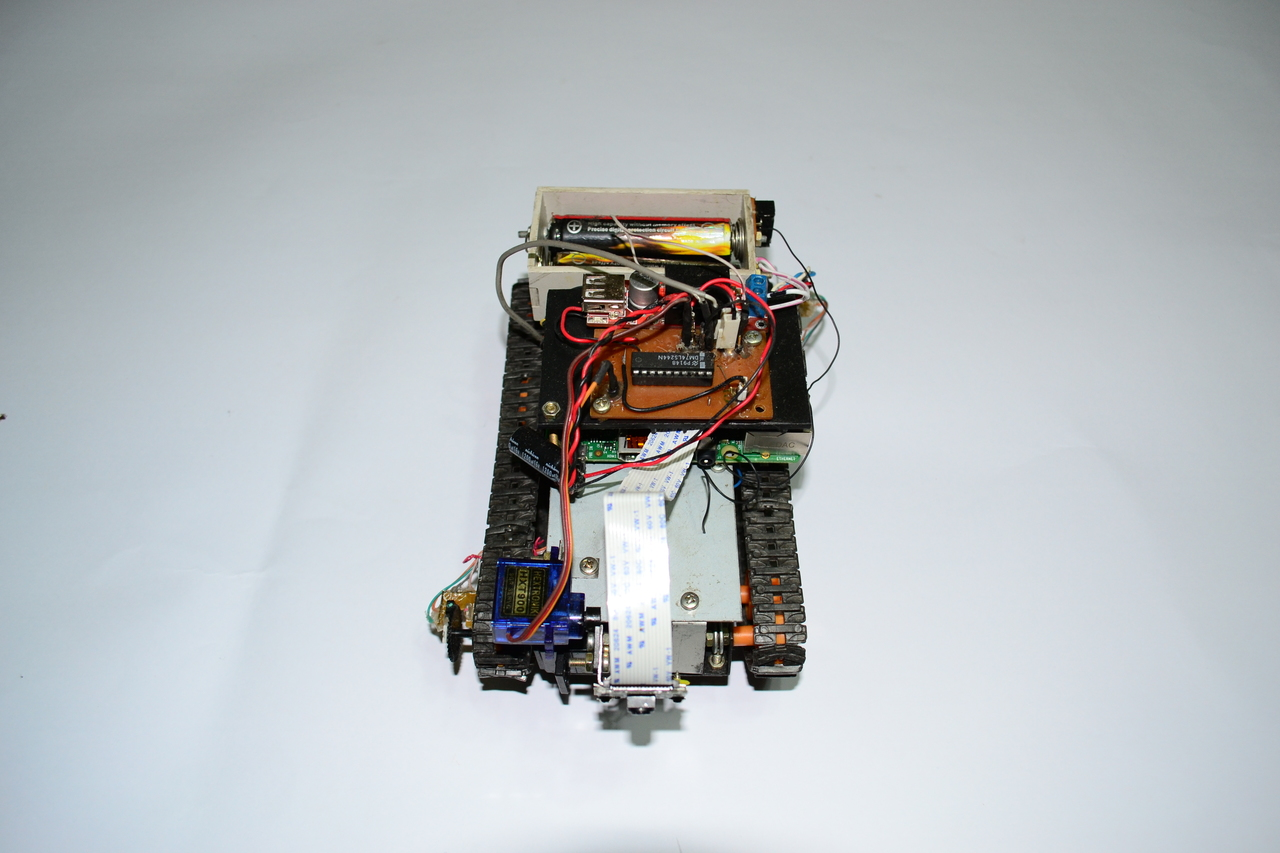
\includegraphics[width=0.8\textwidth]{r-DSC_0009.JPG}
    \caption{Vista frontal del robot. Se observa: el distribuidor de energ�a y regulador de voltaje al centro.}
\end{figure}

\newpage
\markboth{ANEXOS}{ANEXO C}
\addcontentsline{toc}{section}{Anexo C: Planilllas de seguimiento de sprint}
\section*{Anexo C: Planilllas de seguimiento de sprint}

\begin{table}
\centering
\begin{tabular}{|c|l|c|l|c|c|c|c|c|c|c|c|c|c|}
\hline
\multicolumn{4}{|r|}{} & 
V & L & M & X & J & V & L & M & X & J \\
\hline
\multicolumn{4}{|r|}{} & 
\rotatebox[origin=c]{90}{26-sep} & 
\rotatebox[origin=c]{90}{29-sep} & 
\rotatebox[origin=c]{90}{30-sep} & 
\rotatebox[origin=c]{90}{01-oct} & 
\rotatebox[origin=c]{90}{02-oct} & 
\rotatebox[origin=c]{90}{03-oct} & 
\rotatebox[origin=c]{90}{06-oct} & 
\rotatebox[origin=c]{90}{07-oct} & 
\rotatebox[origin=c]{90}{08-oct} & 
\rotatebox[origin=c]{90}{09-oct} \\
\hline
\multicolumn{4}{|r|}{\textbf{Tareas pendientes}} & 
9 & 8 & 8 & 8 & 8 & 5 & 4 & 2 & 2 & 2 \\
\hline
\multicolumn{4}{|r|}{\textbf{Horas pendientes}} & 
74 & 71 & 71 & 77 & 69 & 61 & 53 & 45 & 37 & 31 \\
\hline
\textbf{US} & \textbf{Tarea} & \textbf{Tipo} & \textbf{Estado} &
\multicolumn{10}{|c|}{\textbf{Esfuerzo}}\\
\hline
US1 &
T1 & Implementaci�n & Completada &
0 & 0 & 0 & 0 & 0 & 0 & 0 & 0 & 0 & 0 \\ 
\hline
US1 &
T2  & Investigaci�n & Completada &
0 & 0 & 0 & 0 & 0 & 0 & 0 & 0 & 0 & 0 \\ 
\hline
US1 &
T3 & Configuraci�n & Completada &
2 & 0 & 0 & 0 & 0 & 0 & 0 & 0 & 0 & 0 \\ 
\hline
US1 &
T4  & Investigaci�n & Completada &
0 & 0 & 0 & 0 & 0 & 0 & 0 & 0 & 0 & 0 \\ 
\hline
US1 &
T5  & Investigaci�n & Completada &
0 & 0 & 0 & 0 & 0 & 0 & 0 & 0 & 0 & 0 \\ 
\hline
US1 &
T6  & Implementaci�n & Completada &
5 & 4 & 4 & 10 & 2 & 0 & 0 & 0 & 0 & 0 \\
\hline
US1 &
T7  & Implementaci�n & Completada &
2 & 2 & 2 & 2 & 2 & 0 & 0 & 0 & 0 & 0 \\
\hline
US1 &
T8 & Pruebas & Completada &
2 & 2 & 2 & 2 & 2 & 0 & 0 & 0 & 0 & 0 \\
%--------
\hline
US2 &
T1  & Implementaci�n & Completada &
8 & 8 & 8 & 8 & 8 & 6 & 0 & 0 & 0 & 0 \\ 
\hline
US2 &
T2  & Implementaci�n & Completada &
8 & 8 & 8 & 8 & 8 & 8 & 6 & 0 & 0 & 0 \\ 
\hline
US2 &
T3  & Pruebas & Completada &
2 & 2 & 2 & 2 & 2 & 2 & 2 & 0 & 0 & 0 \\
%--------------------------------------------------------------------
\hline
US3 &
T1  & Implementaci�n & Pendiente &
20 & 20 & 20 & 20 & 20 & 20 & 20 & 20 & 12 & 6 \\
\hline
US3 &
T2  & Implementaci�n & Pendiente &
25 & 25 & 25 & 25 & 25 & 25 & 25 & 25 & 25 & 25 \\
\hline

\end{tabular}
\caption{Planilla de seguimiento del sprint A}
\label{table:planillaSPA}
\end{table}
%\end{landscape}
%\end{document}



  \bookmark[page=13,level=-1]{Índice de cuadros}

\end{document}
